\documentclass [a4paper,12pt]{book}
\usepackage[italian]{babel}
\usepackage[utf8]{inputenc}
\usepackage[T1]{fontenc}
\usepackage{lmodern}
\usepackage{graphicx}
\usepackage{fancyhdr}
\usepackage{float}
\restylefloat{table,figure}
\usepackage{url}
\usepackage[bookmarks,pdftex,
pdfauthor={Giovanni Ricucci},
pdftitle={Progetto Ingegneria del Software},
pdfsubject={Relazione},
pdfkeywords={},
pdfproducer={Latex with hyperref},
pdfcreator={pdflatex}]{hyperref}
\usepackage{booktabs}
\title{Doodle: Pianificazione eventi}
\author{Giovanni Ricucci}
\date{\today}
\begin{document}
\frontmatter
\maketitle
\pagestyle{headings}
\tableofcontents
\mainmatter
\chapter{Requisiti Funzionali}

L'applicazione deve permettere di creare eventi e di gestire le disponibilità espresse dagli utenti relativamente agli eventi stessi.
Nello specifico, l'applicazione dovrà permettere agli utenti di: 
\begin{enumerate}
\item Creare e gestire un evento (funzionalità riservate agli utenti registrati);
\item Esprimere le proprie disponibilità per un dato evento (funzionalità disponibile sia per utenti registrati sia per utenti non registrati). 
\end{enumerate}

\chapter{Scenari}

\begin{enumerate}
\item L'applicazione deve poter registrare nuovi utenti ,oltre a quelli registrati, e fare delle ricerche su utenti già registrati:
\begin{itemize}
\item Il sistema richiede le credenziali d accesso all'utente se questo è registrato;
\item Se l'utente è registrato può procedere con l'accesso;
\item Se l'utente vuole registrarsi all'applicazione fornisce i dati personali;
\item I dati personali richiesti sono: nome, nickname, password ed email (opzionale);
\item Una volta registrato l'utente non potrà più modificare i propri dati;
\item Non è previsto nessun meccanismo di recupero della password; 
\end{itemize}
\item L'applicazione permetterà un meccanismo di autenticazione degli utenti:
\begin{itemize}
\item L'utente fornisce le proprie credenziali d'accesso (nickname e password) al sistema;
\item Il sistema concede l'accesso, se l'utente è stato riconosciuto;
\item Dopo aver effettuato l'accesso, l'utente/amministratore vede elencati tutti gli eventi da lui creati;
\item L'utente/amministratore può in ogni momento chiudere l'evento da lui creato eventualmente fornendo i motivi;
\item L'utente/amministratore può in ogni momento cancellare il sondaggio da lui creato rendendolo inaccessibile.
\end{itemize}
\item L'utente registrato all'applicazione deve poter creare e gestire eventi :
\begin{itemize}
\item L' utente fornisce i dati necessari e opzionali alla creazione dell'evento;
\item I dati necessari sono: nome dell'evento e opzioni di scelta (giorni e orari);
\item I dati opzionali sono: luogo dell'evento e descrizione dell'evento;
\item Durante la creazione di un evento, ogni opzione di scelta deve essere cancellabile o modificabile;
\item Una volta che l'evento è stato creato, non è più possibile modificarlo;
\item Al termine della fase di creazione il sistema comunica un identificatore univoco dell'evento creato. Tale identificatore verrà usato in seguito per gestire l'evento;
\item Dopo averlo creato, il sistema iscrive automaticamente l'utente all'evento;
\item Al termine della creazione l'evento diventa automaticamente disponibile per qualunque utente volesse esprime la sua disponibilità;
\end{itemize}
\item L'applicazione deve permettere agli utenti di poter accedere, visualizzare le informazioni, poter iscriversi ed esprimere le proprie disponibilità per ogni evento:
\begin{itemize}
\item L' utente che accede a un evento può visualizzare le disponibilità di tutti gli altri utenti e i commenti già inseriti;
\item L' utente che accede a un evento può inserire il proprio nome e la disponibilità (si/no);
\item Nel caso l'evento è stato chiuso può visualizzare i motivi che sono stati eventualmente scelti dall'utente/amministratore di quel evento;
\item Se l'utente accede all'evento dopo aver effettuato l'accesso, il suo nome e il suo nickname saranno inseriti nell'apposito modulo in automatico;
\item Se l'utente accede all'evento dopo aver effettuato l'accesso può lasciare un commento e modificare le proprie disponibilità;
\end{itemize}

\end{enumerate}


\chapter{Diagramma dei casi d'uso}

\section{Registrazione}
\begin{figure}[h!]
\centering
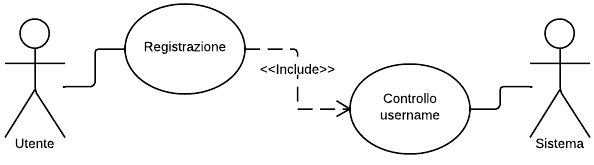
\includegraphics[scale=0.60]{img/use/Reg.png}
\caption{Registrazione}
\label{fig:registrazione}
\end{figure}
\begin{table}[H]
\begin{tabular}{p{0.35\textwidth}|p{0.65\textwidth}}
\toprule
NOME & Registrazione;\\
\hline
OBBIETTIVO: & Registrare l utente nella applicazione;\\
\hline
PRE-CONDIZIONE & L'utente non deve essere registrato nel sistema;\\
\hline
SUCCESSO: & La registrazione avviene con successo;\\
\hline
FALLIMENTO: & Non è possibile effettuare la registrazione; \\
\hline
ATTORE PRIMARIO: & Utente;\\
\hline
ATTORI SECONDARI: & Sistema;\\
\bottomrule
\end{tabular}
\caption{Registrazione Utente}
\label{table:reg}
\end{table}
FLUSSO PRINCIPALE:
\begin{enumerate}
\item L'utente compila e inoltra il modulo d'iscrizione;
\begin{enumerate}
\item Controllo dei campi non opzionali e necessari alla registrazione;
\item Doppio inserimento password;
\end{enumerate}
\item Controllo del username;
\item Ricerca del username;
\begin{enumerate}
\item Il sistema verifica che l'utente (username univoco) non sia già registrato;
\end{enumerate}
\item Avviene la registrazione del utente;
\item La registrazione è avvenuta con successo;
\end{enumerate}

\section{Login}
\begin{figure}[h!]
\centering
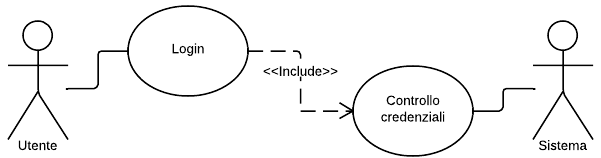
\includegraphics[scale=0.50]{img/use/Log.png}
\caption{Login}
\label{fig:Login}
\end{figure}
\begin{table}[H]
\begin{tabular}{p{0.35\textwidth}|p{0.65\textwidth}}
\toprule
NOME & Login;\\
\hline
OBBIETTIVO: & Ottenere accesso all'applicazione;\\
\hline
PRE-CONDIZIONE & L'utente deve essere registrato all'applicazione;\\
\hline
SUCCESSO: & L'utente ottiene accesso all'applicazione;\\
\hline
FALLIMENTO: & La procedura non va a buon fine;\\
\hline
ATTORE PRIMARIO: & Utente;\\
\hline
ATTORI SECONDARI: & Sistema;\\
\bottomrule
\end{tabular}
\caption{Login Utente}
\label{table:log}
\end{table}
FLUSSO PRINCIPALE:
\begin{enumerate}
\item L'utente immette le proprie credenziali;
\item L'utente inoltra la richiesta di accesso;
\begin{enumerate}
\item Il sistema verifica la corrispondenza delle credenziali;
\end{enumerate}
\item L'utente ottiene accesso al' applicazione;
\end{enumerate}

\section{Crea Evento}
\begin{figure}[h!]
\centering
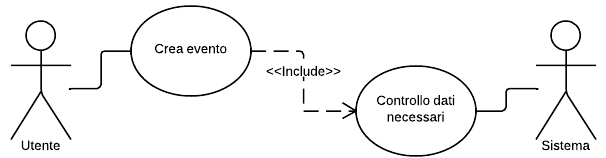
\includegraphics[scale=0.60]{img/use/creaevento.png}
\caption{Crea evento}
\label{fig:creaeve}
\end{figure}
\begin{table}[H]
\begin{tabular}{p{0.35\textwidth}|p{0.65\textwidth}}
\toprule
NOME & Crea evento;\\
\hline
OBBIETTIVO: & Creare un evento;\\
\hline
PRE-CONDIZIONE & L'utente deve essere registrato all'applicazione;
L'utente deve aver eseguito l'accesso all'applicazione;\\
\hline
SUCCESSO: & L'utente crea l'evento;\\
\hline
FALLIMENTO: & La procedura non va a buon fine;\\
\hline
ATTORE PRIMARIO: & Utente;\\
\hline
ATTORI SECONDARI: & Sistema;\\
\bottomrule
\end{tabular}
\caption{Crea evento}
\label{table:creaevento}
\end{table}
FLUSSO PRINCIPALE:
\begin{enumerate}
\item L'utente immette i dati necessari alla creazione dell'evento;
\item L'utente inoltra la richiesta di creazione;
\begin{enumerate}
\item Il sistema verifica i dati inseriti;
\end{enumerate}
\item L'utente ha creato l'evento;
\end{enumerate}

\section{Partecipazione ad evento – Utente senza accesso}
\begin{figure}[h!]
\centering
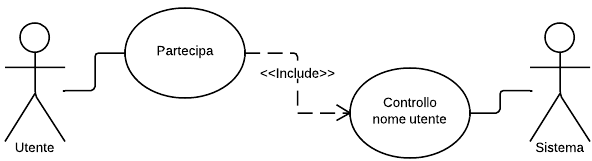
\includegraphics[scale=0.60]{img/use/PartecipaSa.png}
\caption{Partecipazione senza accesso}
\label{fig:ParteSA}
\end{figure}

\begin{table}[H]
\begin{tabular}{p{0.35\textwidth}|p{0.65\textwidth}}
\toprule
NOME & Partecipazione ad evento senza accesso;\\
\hline
OBBIETTIVO: & L'utente rende la propria disponibilità per un evento senza essere registrato all'applicazione;\\
\hline
PRE-CONDIZIONE & Nessuna;\\
\hline
SUCCESSO: & L'utente si rende disponibile per tale evento;\\
	\hline
FALLIMENTO: & La procedura non va a buon fine;\\
\hline
ATTORE PRIMARIO: & Utente;\\
\hline
ATTORI SECONDARI: & Sistema;\\
\bottomrule
\end{tabular}
\caption{Partecipazione ad evento senza accesso}
\label{table:parSA}
\end{table}
FLUSSO PRINCIPALE:
\begin{enumerate}
\item L'utente seleziona l'evento desiderato e visualizza tutte le informazioni riguardanti l'evento;
\begin{enumerate}
\item L'utente visualizza la lista di tutti gli utenti iscritti all'evento e il username dell'utente che l ha creato;
\item L'utente visualizza la lista di tutti i commenti per l evento selezionato;
\end{enumerate}
\item L'utente inserisce il proprio nome nel apposito spazio;
\begin{enumerate}
\item Il sistema verifica che l'utente ha inserito correttamente il suo nome;
\end{enumerate}
\item L'utente inoltra la richiesta d iscrizione;
\item L'Utente si rende disponibile per tale evento;
\end{enumerate}

\section{Partecipazione ad evento – Utente con accesso}
\begin{figure}[h!]
\centering
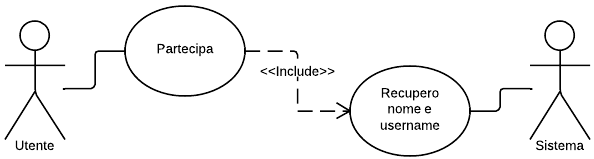
\includegraphics[scale=0.60]{img/use/PartecipaCa.png}
\caption{Partecipazione con accesso}
\label{fig:ParteCA}
\end{figure}
\begin{table}[H]
\begin{tabular}{p{0.35\textwidth}|p{0.65\textwidth}}
\toprule
NOME & Partecipazione ad evento con accesso;\\
\hline
OBBIETTIVO: & L'utente rende la propria disponibilità per un evento dopo aver eseguito l'accesso all'applicazione;\\
\hline
PRE-CONDIZIONE & L'utente deve essere registrato all'applicazione;\\
\hline
SUCCESSO: & L'utente si rende disponibile per tale evento;\\
\hline
FALLIMENTO: & La procedura non va a buon fine;\\
\hline
ATTORE PRIMARIO: & Utente;\\
\hline
ATTORI SECONDARI: & Sistema;\\
\bottomrule
\end{tabular}
\caption{Partecipazione ad evento con accesso}
\label{table:par2}
\end{table}
FLUSSO PRINCIPALE:
\begin{enumerate}
\item L'utente seleziona l'evento desiderato e visualizza tutte le informazioni riguardanti l'evento;
\begin{enumerate}
\item L'utente visualizza la lista di tutti gli utenti iscritti all'evento e il username dell'utente che l ha creato;
\item L'Utente visualizza la lista di tutti i commenti per l evento selezionato;
\end{enumerate}
\item L'utente inoltra la richiesta d iscrizione;
\begin{enumerate}
\item Il Sistema recupera il nome del utente che ha eseguito l accesso;
\item Il Sistema recupera il username del utente che ha eseguito l accesso;
\end{enumerate}
\item L'utente si rende disponibile per tale evento;
\begin{enumerate}
\item L'utente può lasciare commenti per l evento selezionato;
\end{enumerate}
\end{enumerate}

\section{Chiudere evento}
\begin{figure}[H]
\centering
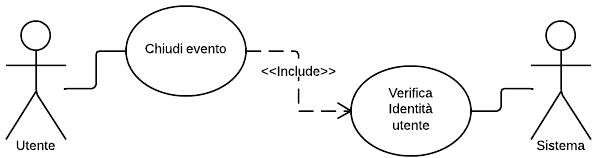
\includegraphics[scale=0.60]{img/use/Chiude.png}
\caption{Chiudere un evento}
\label{fig:Chiudere}
\end{figure}
\begin{table}[H]
\begin{tabular}{p{0.35\textwidth}|p{0.65\textwidth}}
\toprule
NOME & Chiusura di un evento;\\
\hline
OBBIETTIVO: & L utente chiude un evento;\\
\hline
PRE-CONDIZIONE & L'utente deve essere registrato all'applicazione;
L'utente è il creatore dell'evento;\\
\hline
SUCCESSO: & L utente chiude correttamente l evento;\\
\hline
FALLIMENTO: & La procedura non va a buon fine;\\
\hline
ATTORE PRIMARIO: & Utente;\\
\hline
ATTORI SECONDARI: & Sistema;\\
\bottomrule
\end{tabular}
\caption{Chiudere un evento}
\label{table:chiude}
\end{table}	
FLUSSO PRINCIPALE:
\begin{enumerate}
\item L'utente seleziona l'evento desiderato;
\item L'utente inserisce le eventuali cause che hanno portato alla chiusura dell'evento;
\item L'utente inoltra la richiesta di chiusura dell'evento;
\begin{enumerate}
\item Il Sistema controlla che l'utente che vuole chiudere l evento sia il creatore dello stesso;
\end{enumerate}
\item L utente ha chiuso l'evento;
\end{enumerate}

\section{Eliminazione evento}
\begin{figure}[H]
\centering
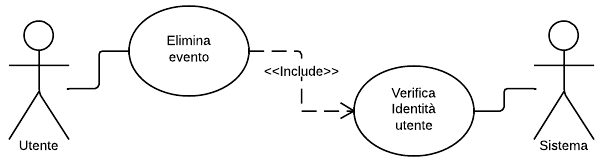
\includegraphics[scale=0.60]{img/use/Elimina.png}
\caption{Eliminare un evento}
\label{fig:Elimina}
\end{figure}
\begin{table}[H]
\begin{tabular}{p{0.35\textwidth}|p{0.65\textwidth}}
\toprule
NOME & Eliminazione di un evento;\\
\hline
OBBIETTIVO: & L'utente elimina un evento;\\
\hline
PRE-CONDIZIONE & L'utente deve essere registrato all'applicazione;
L'utente è il creatore dell'evento;\\
\hline
SUCCESSO: & L utente elimina correttamente l evento;\\
\hline
FALLIMENTO: & La procedura non va a buon fine;\\
\hline
ATTORE PRIMARIO: & Utente;\\
\hline
ATTORI SECONDARI: & Sistema;\\
\bottomrule
\end{tabular}
\caption{Eliminare di un evento}
\label{table:elimina}
\end{table}	
FLUSSO PRINCIPALE:
\begin{enumerate}
\item L'utente seleziona l'evento desiderato;
\item L'utente inoltra la richiesta di eliminazione dell'evento;
\begin{enumerate}
\item Il sistema controlla che l'utente che vuole eliminare l evento sia il creatore dello stesso;
\end{enumerate}
\item L'utente ha eliminato l'evento;
\end{enumerate}

\section{Diagramma casi d'uso completo}
\begin{figure}[H]
\centering
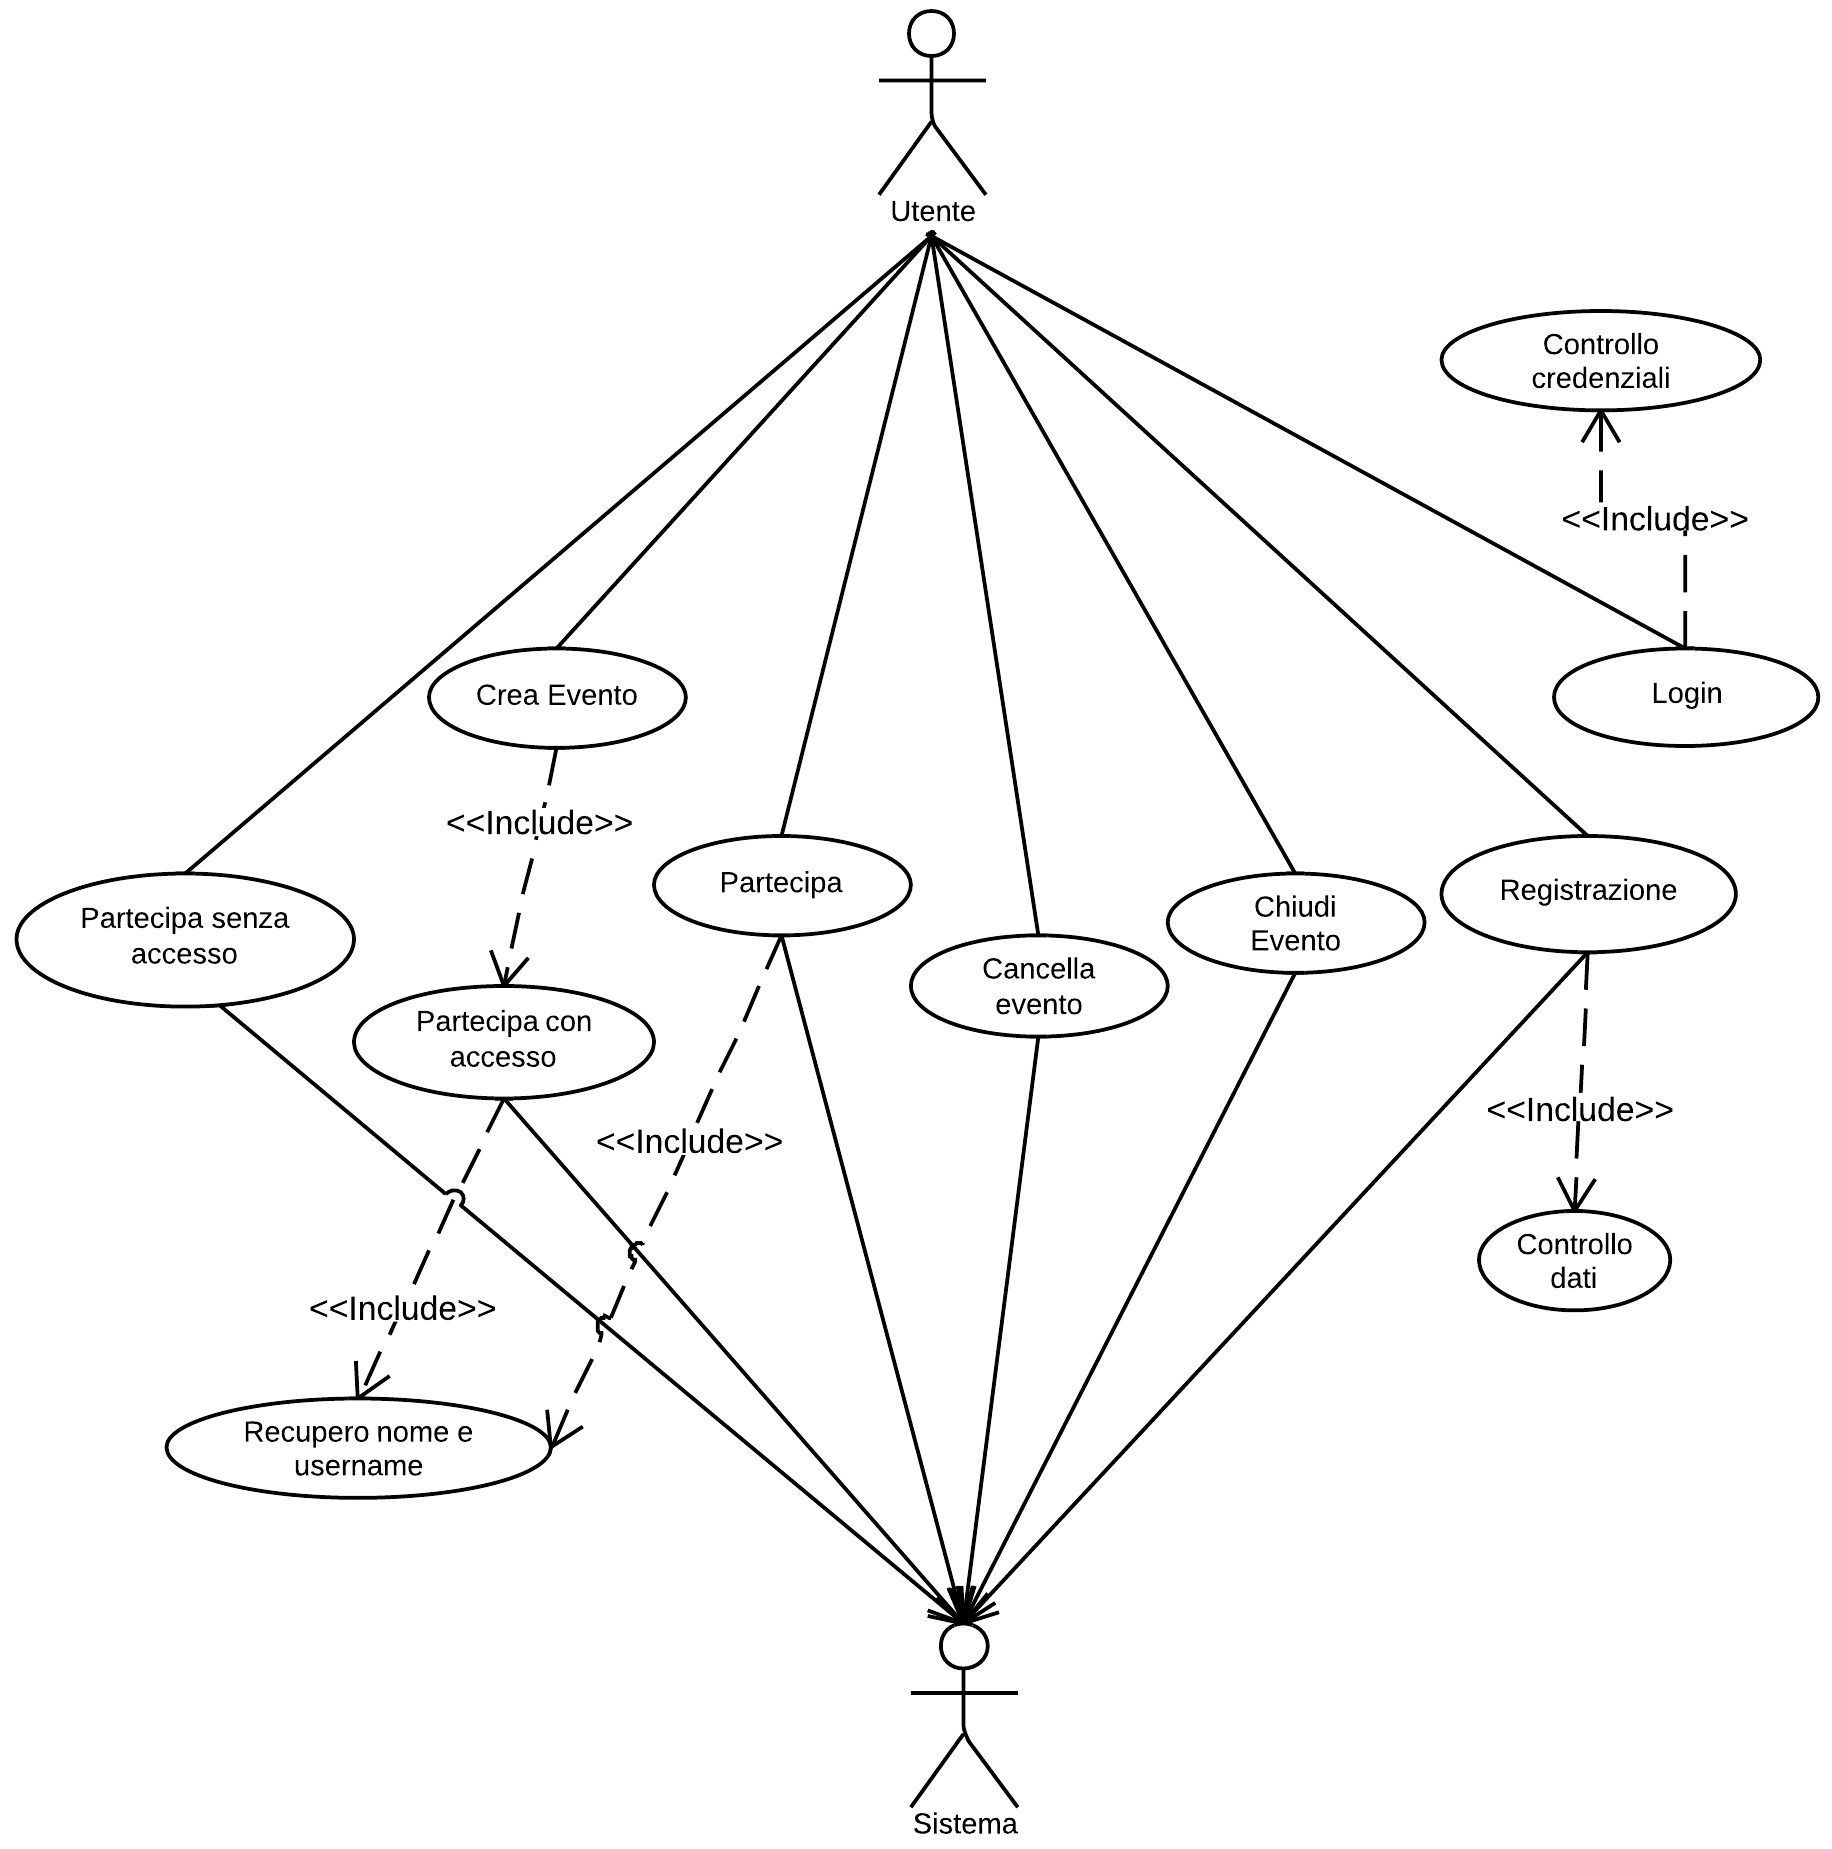
\includegraphics[width=16cm, height=14cm]{img/use/DiagUsocompleto.png}
\caption{Diagramma casi d'uso}
\label{fig:diagcompl}
\end{figure}




\chapter{Diagramma delle attività}

\section{Registrazione}
\begin{figure}[H]
\centering
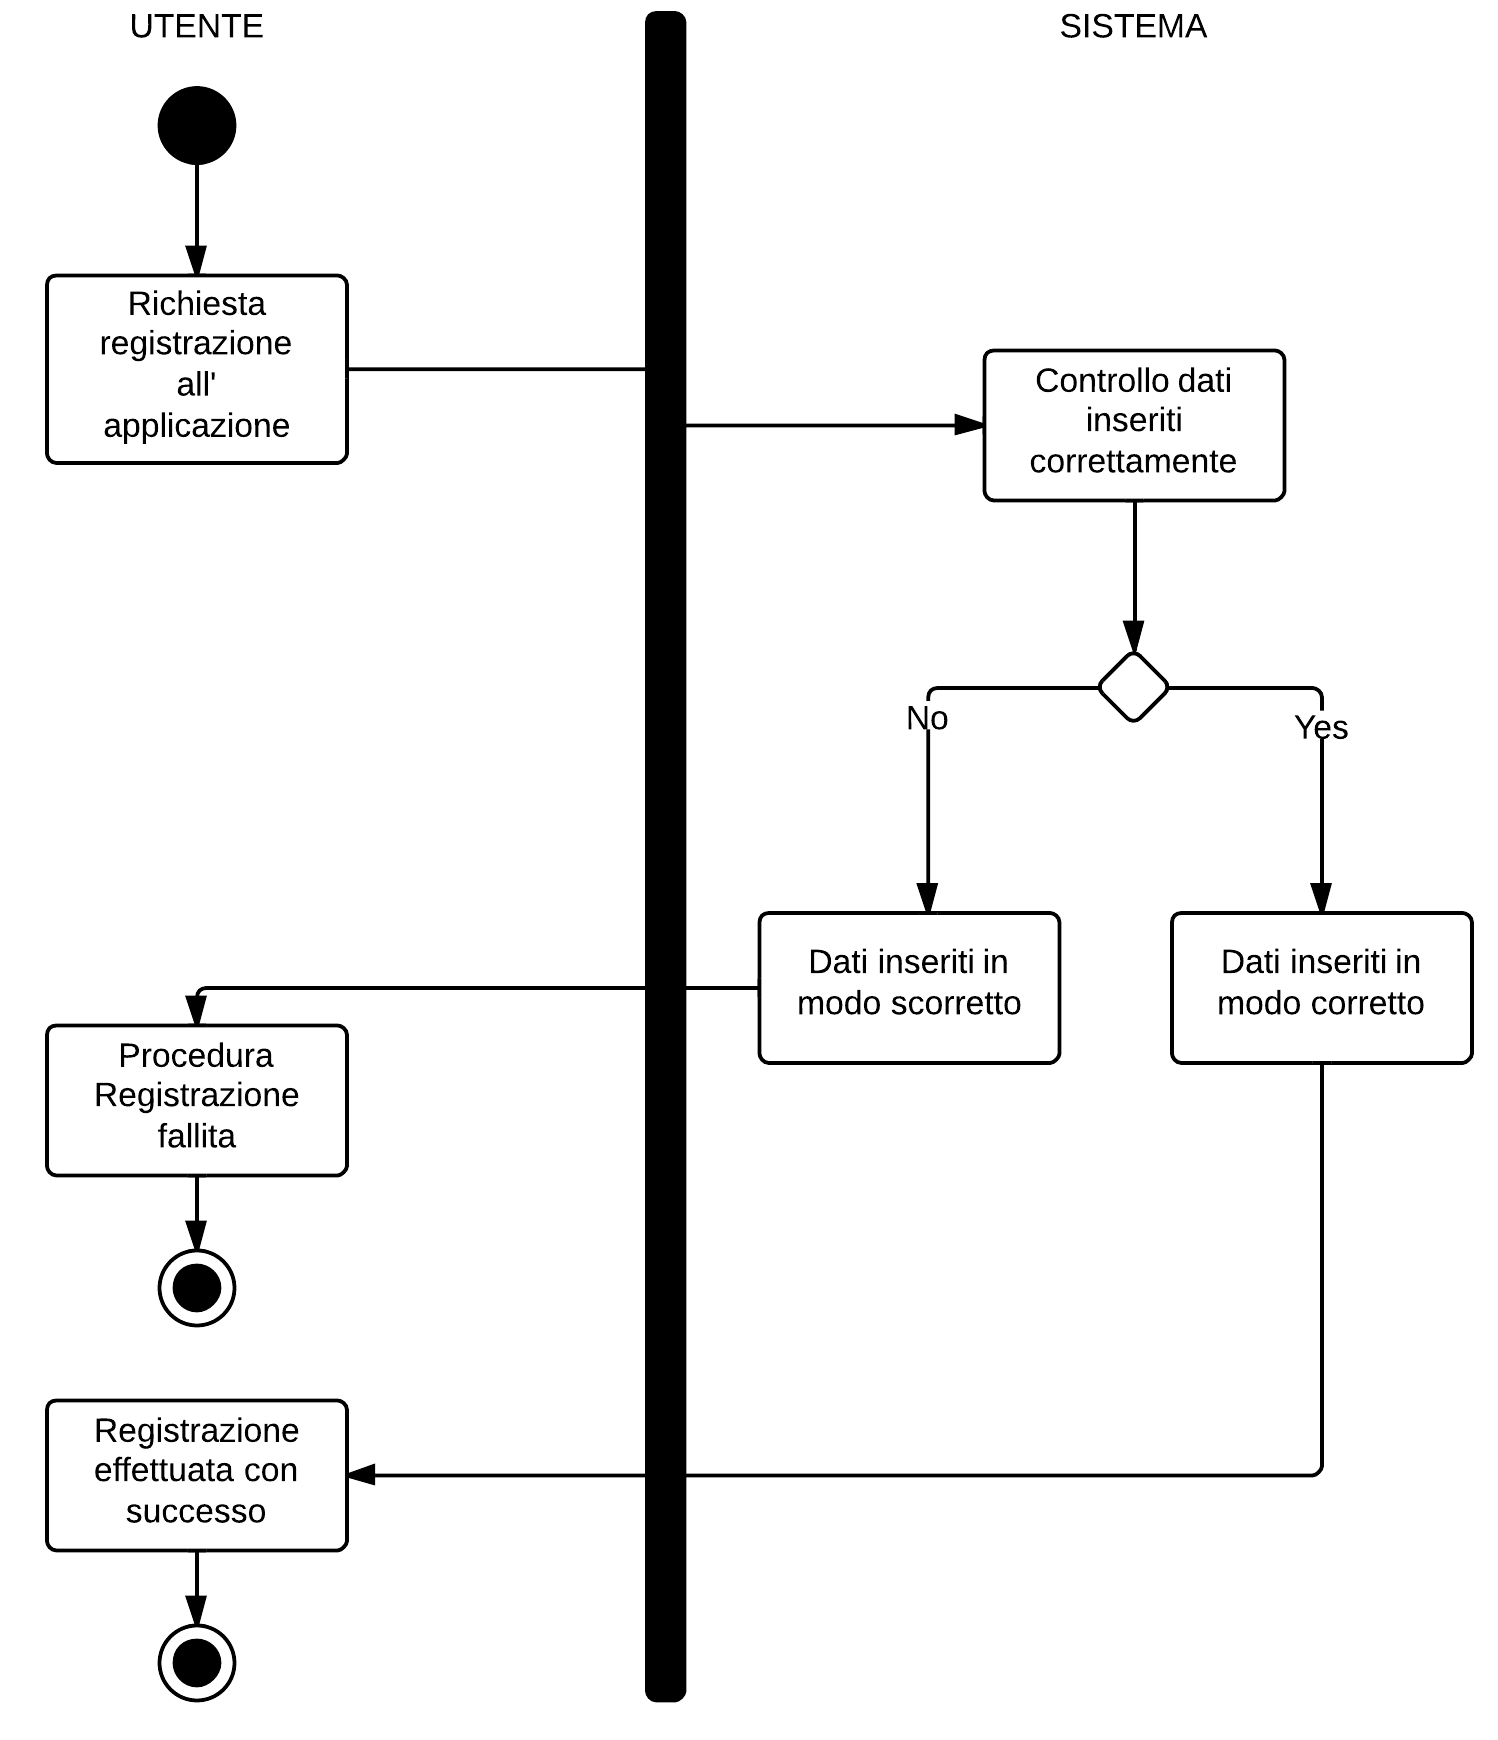
\includegraphics[scale=0.22]{img/activity/Reg.png}
\caption{Diagramma Attività: Registrazione}
\label{fig:attreg}
\end{figure}

\section{Login}
\begin{figure}[H]
\centering
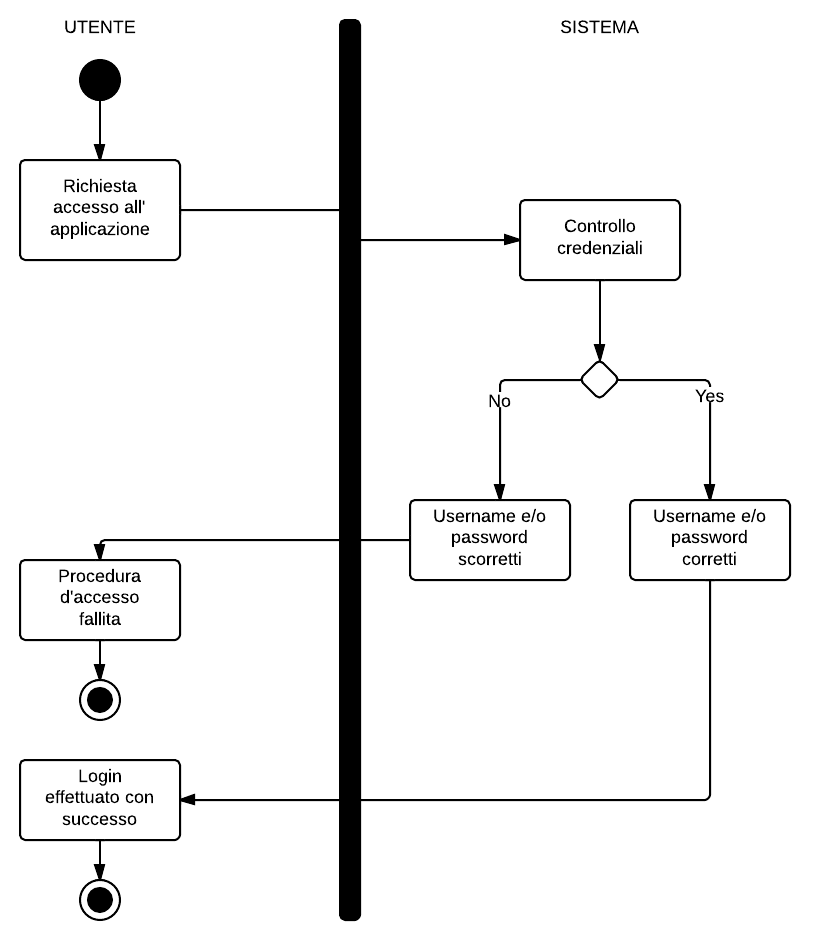
\includegraphics[scale=0.43]{img/activity/Log.png}
\caption{Diagramma Attività: Login}
\label{fig:attlog}
\end{figure}

\section{Crea Evento}
\begin{figure}[H]
\centering
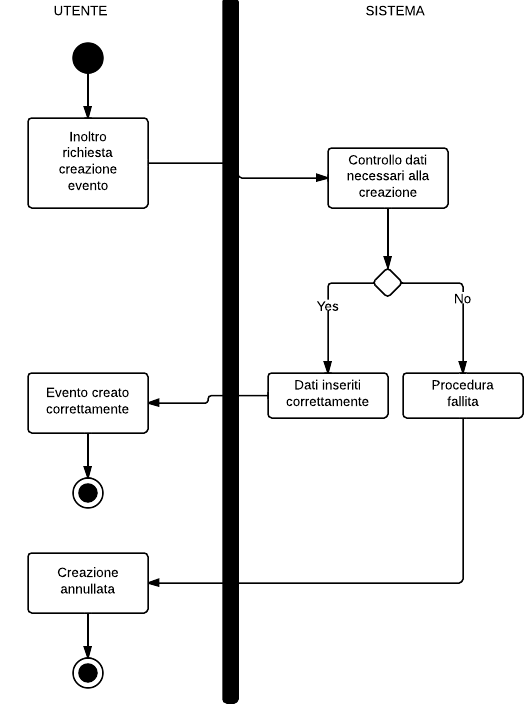
\includegraphics[scale=0.55]{img/activity/crea.png}
\caption{Diagramma Attività: Crea evento}
\label{fig:creaev}
\end{figure}

\section{Partecipazione ad evento – Utente senza accesso}
\begin{figure}[H]
\centering
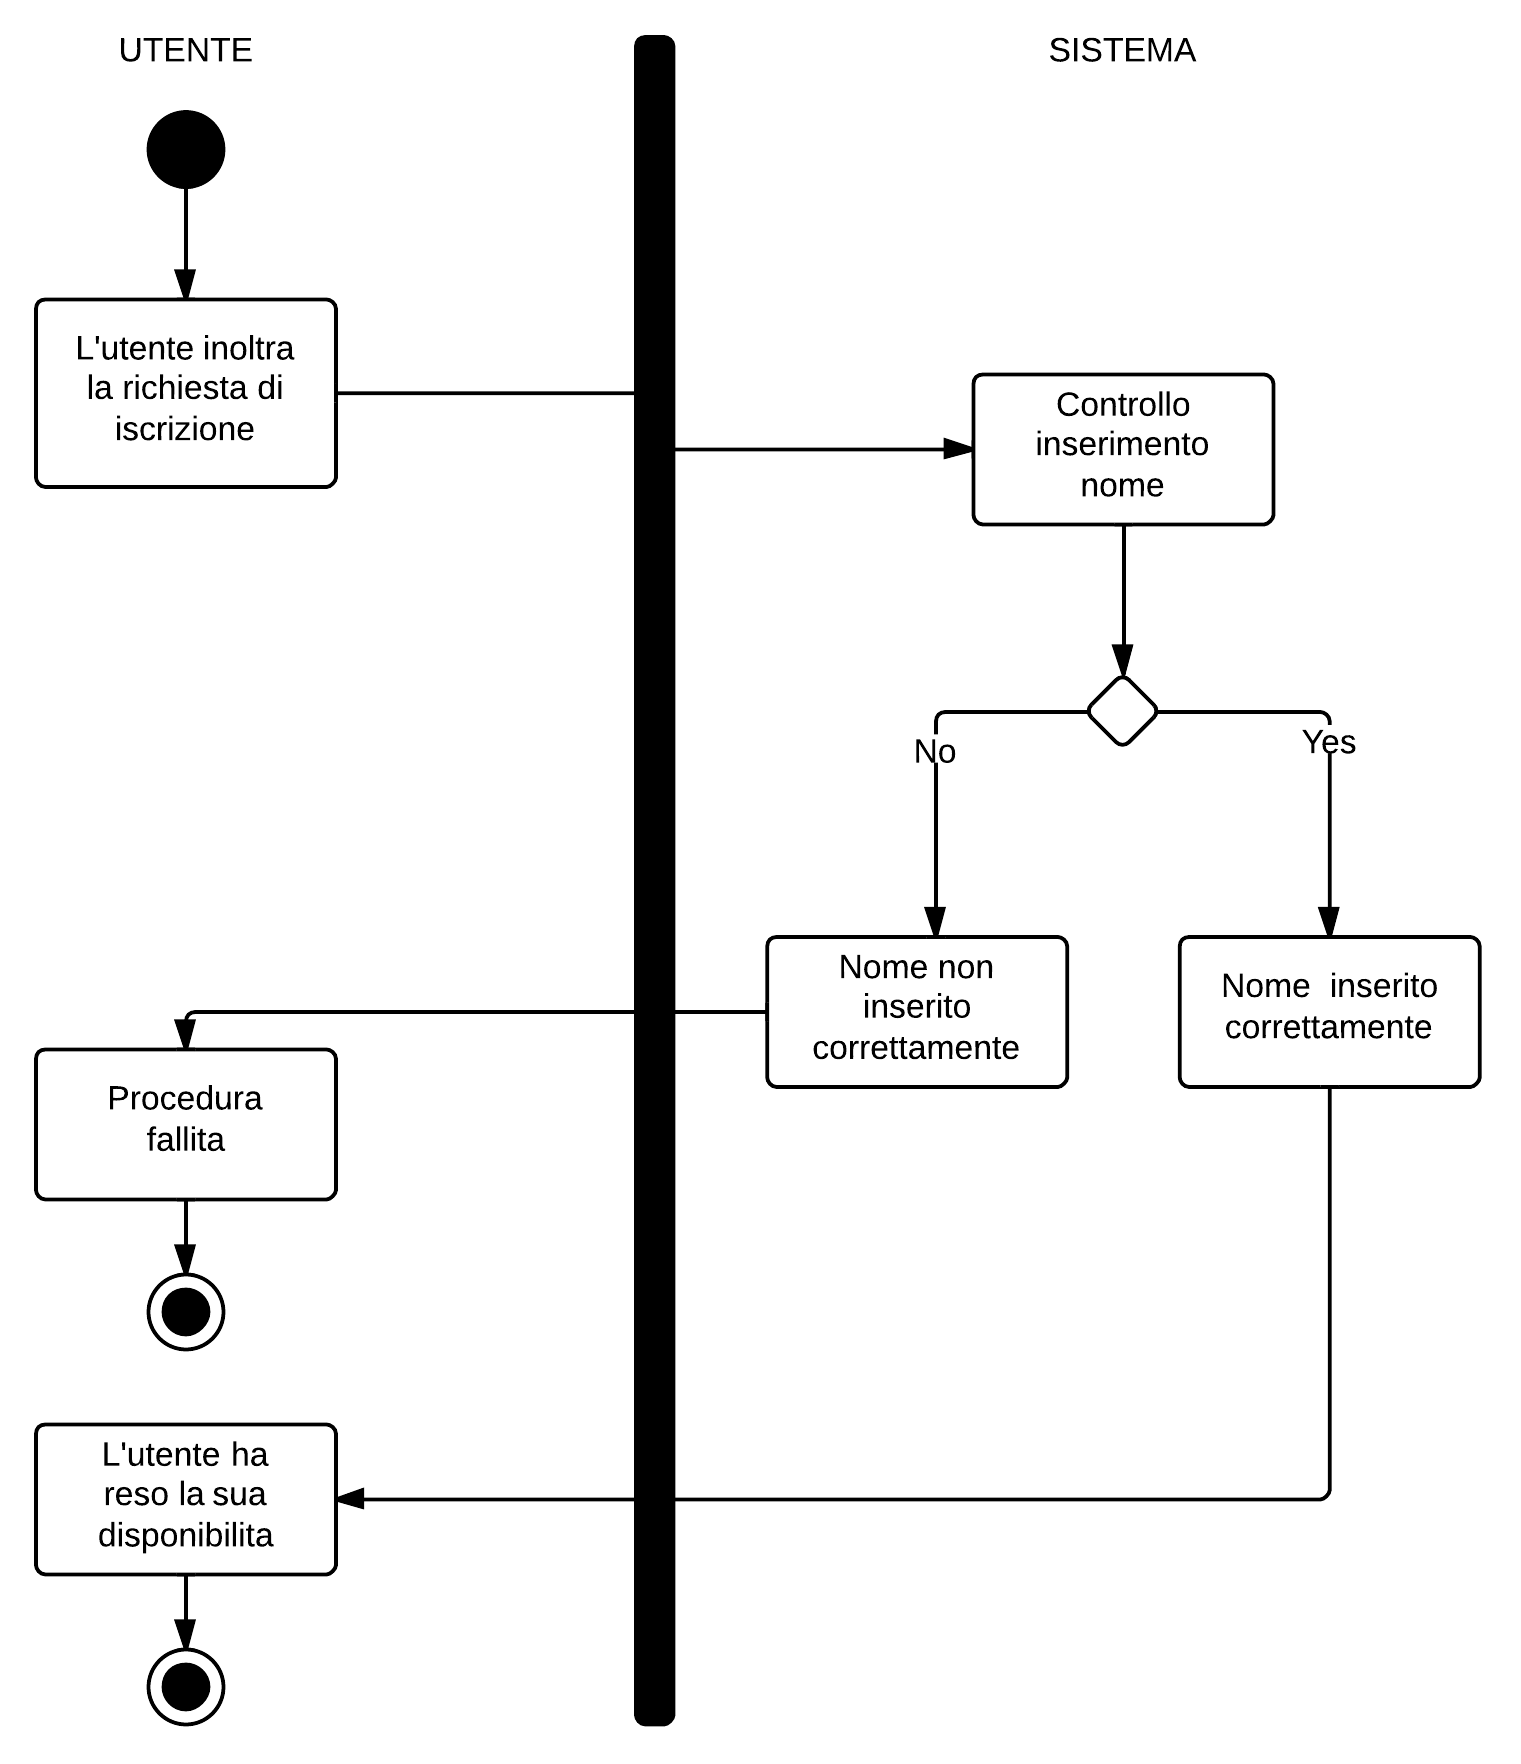
\includegraphics[scale=0.25]{img/activity/PartSa.png}
\caption{Diagramma Attività: Partecipazione senza accesso}
\label{fig:attpartSa}
\end{figure}

\section{Partecipazione ad evento – Utente con accesso}
\begin{figure}[H]
\centering
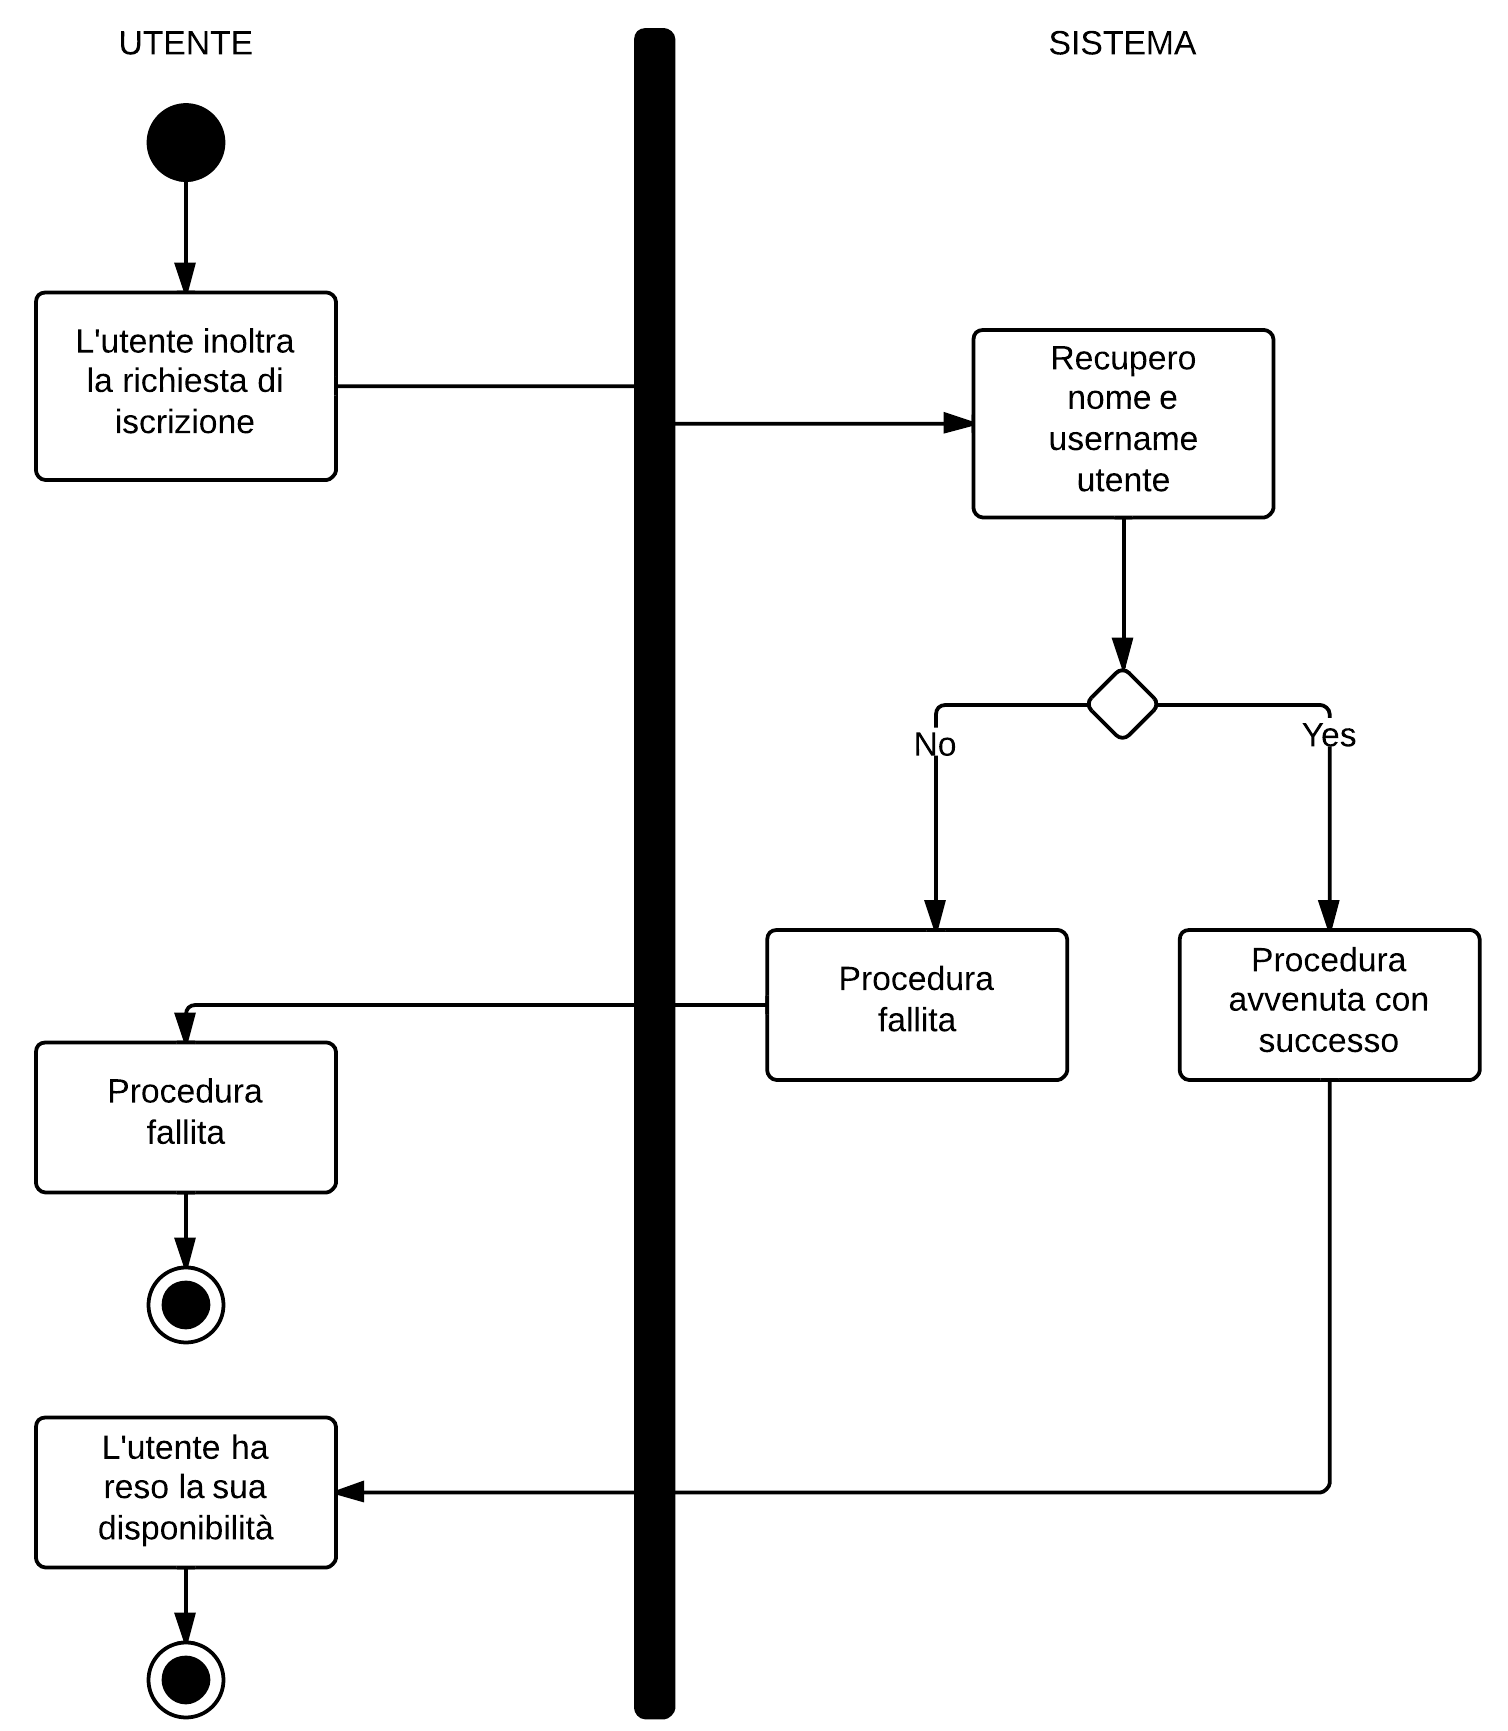
\includegraphics[scale=0.25]{img/activity/PartCa.png}
\caption{Diagramma Attività: Partecipazione con accesso}
\label{fig:attpartCa}
\end{figure}

\section{Chiudere evento}
\begin{figure}[H]
\centering
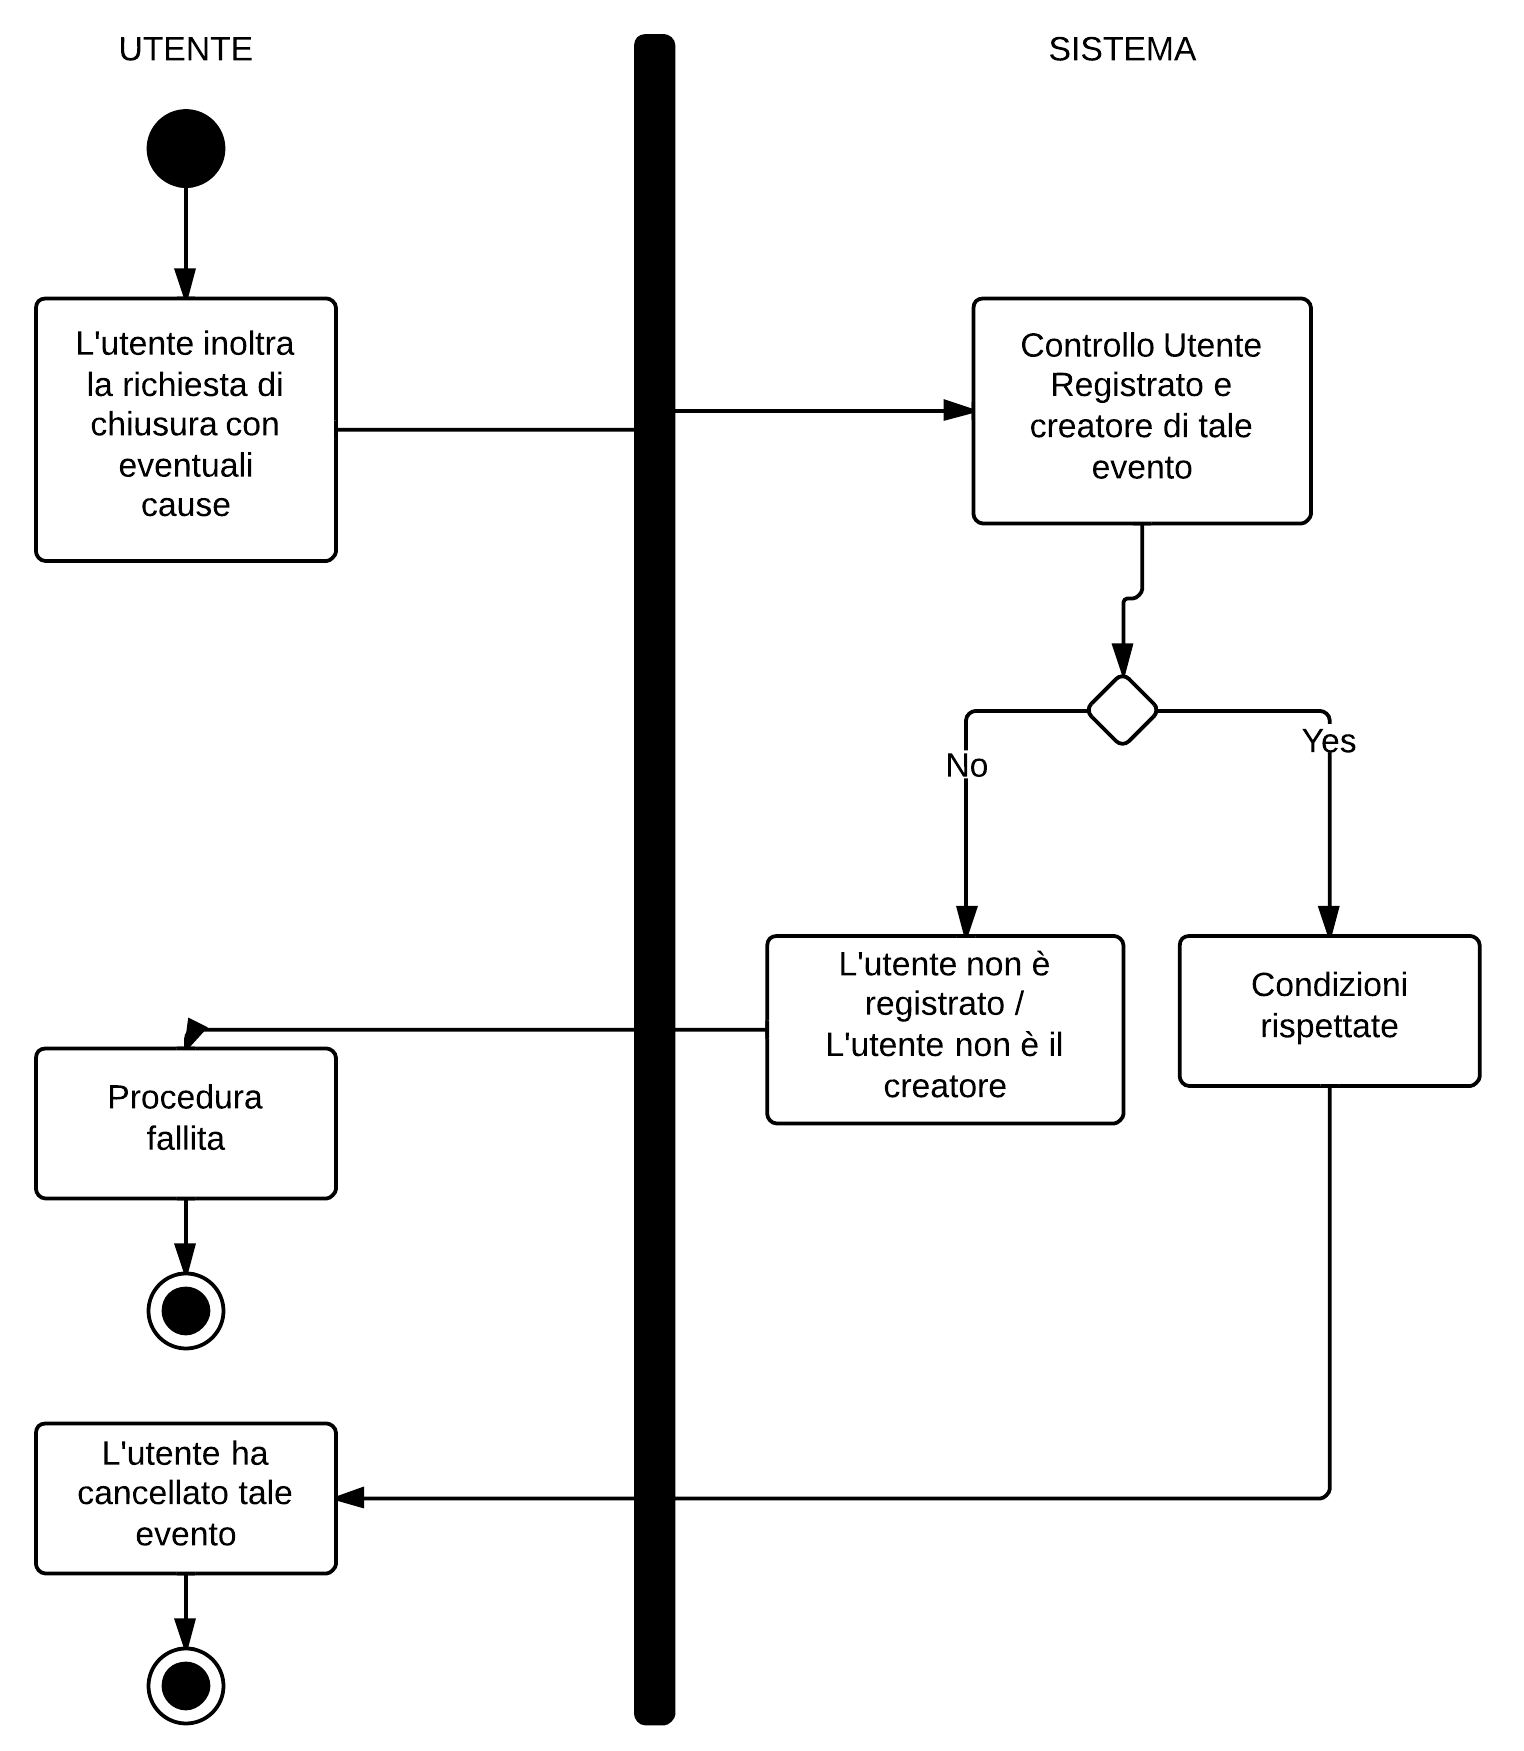
\includegraphics[scale=0.27]{img/activity/chiude.png}
\caption{Chiudere un evento}
\label{fig:attchiude}
\end{figure}

\section{Eliminare evento}
\begin{figure}[H]
\centering
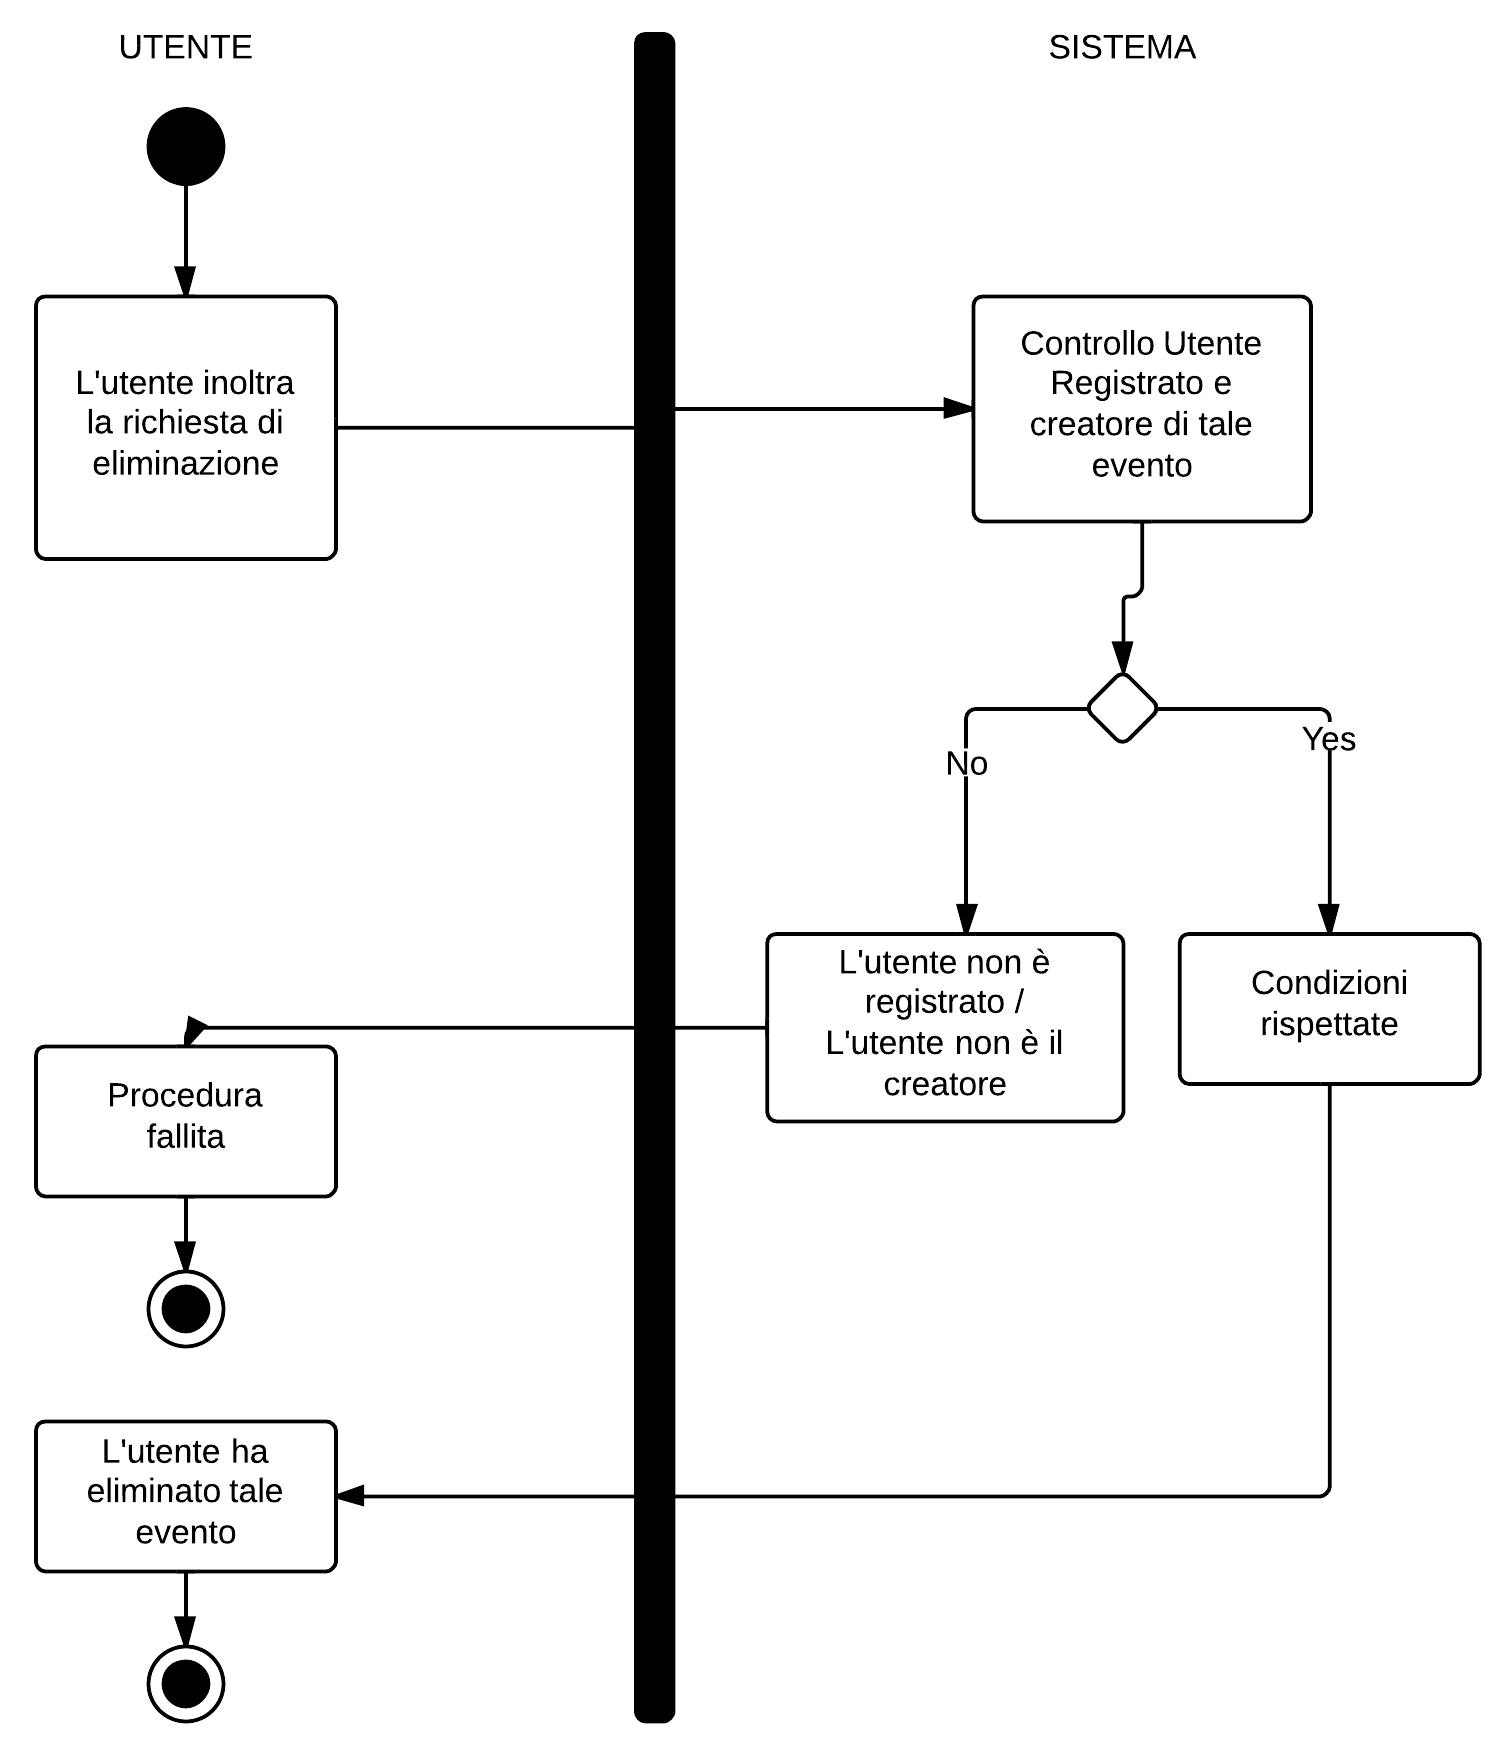
\includegraphics[scale=0.27]{img/activity/elimina.png}
\caption{Eliminare un evento}
\label{fig:accelimina}
\end{figure}
\chapter{Diagramma delle classi}

\section{Cardinalità}
\begin{figure}[H]
\centering
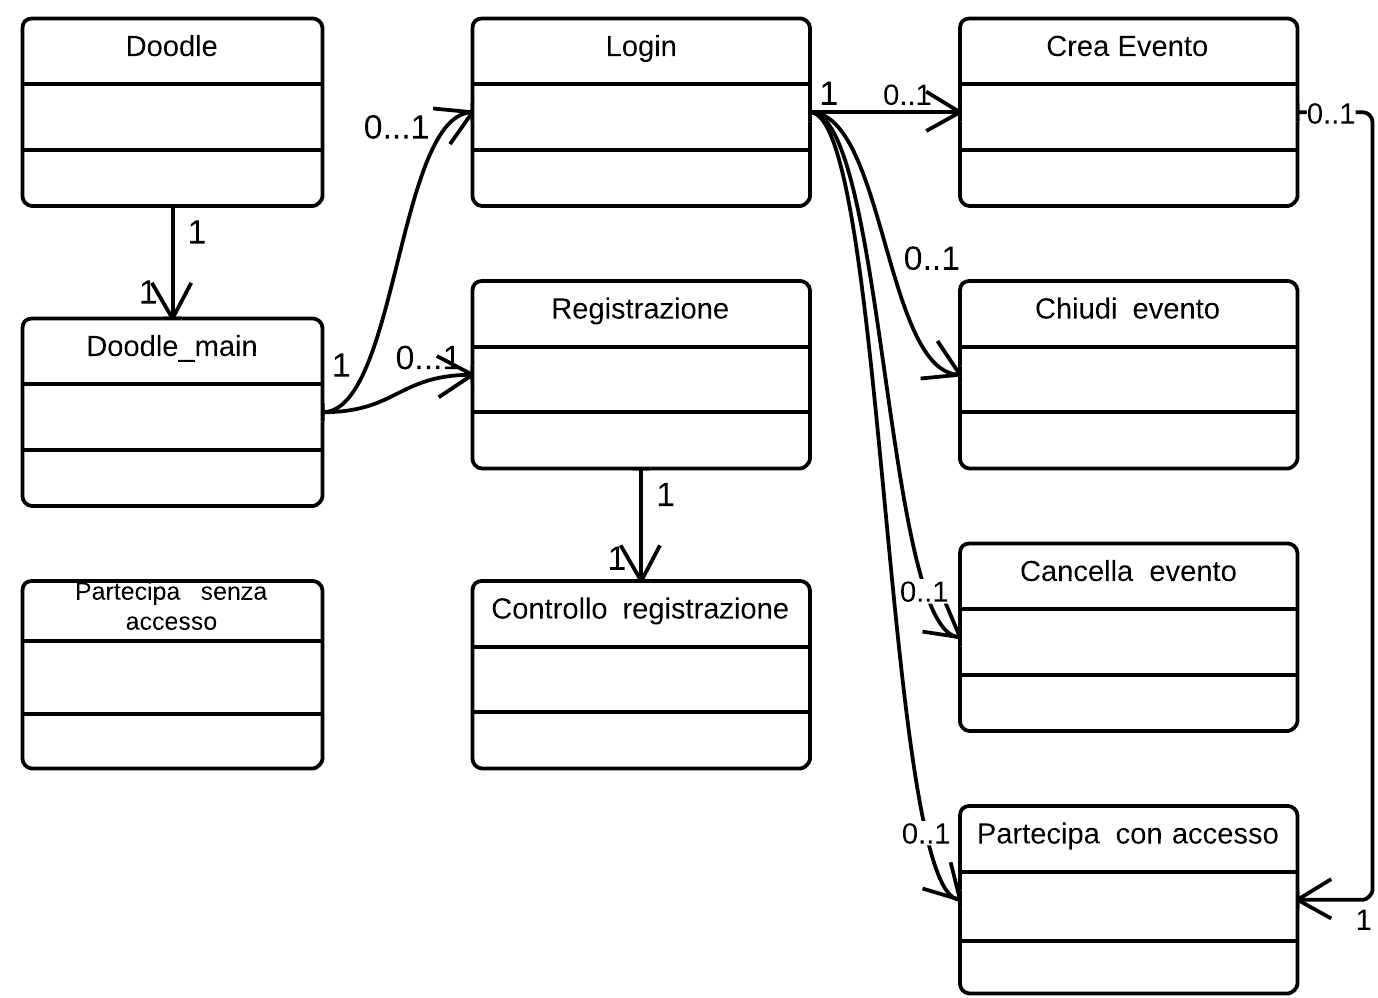
\includegraphics[scale=0.30]{img/classi/classi.png}
\caption{Diagramma delle classi}
\label{fig:classicard}
\end{figure}

\section{Diagramma totale delle classi Doodle}
\begin{figure}[!ht]
\centering
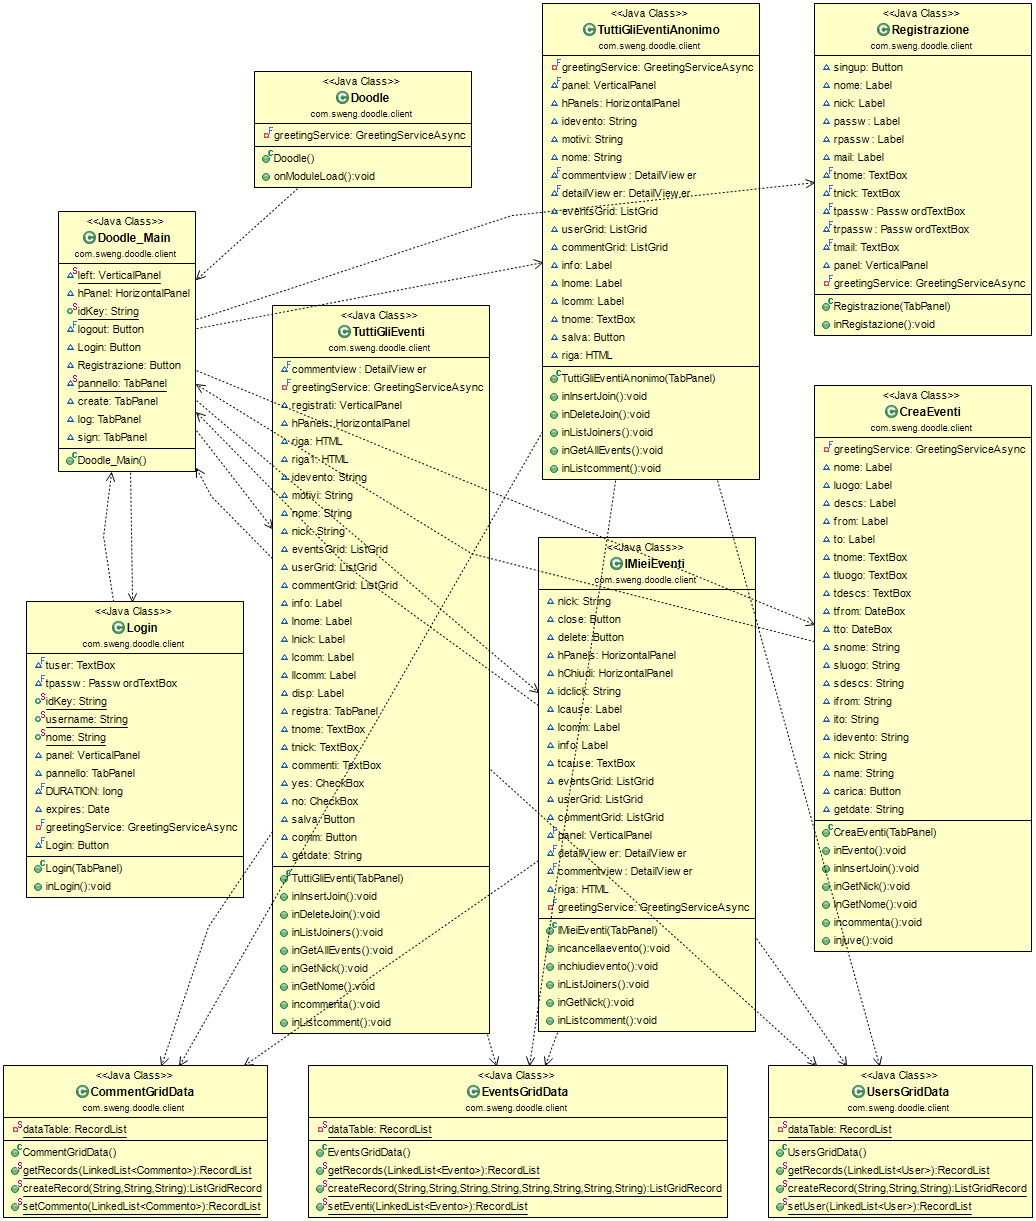
\includegraphics[width=14cm, height=17.2cm]{img/classi/diagrammaclassi.png}
\caption{Diagramma delle classi}
\label{fig:diagclassi}
\end{figure}

\section{Diagramma totale delle classi Doodle 2.0 }
\begin{figure}[!ht]
	\centering
	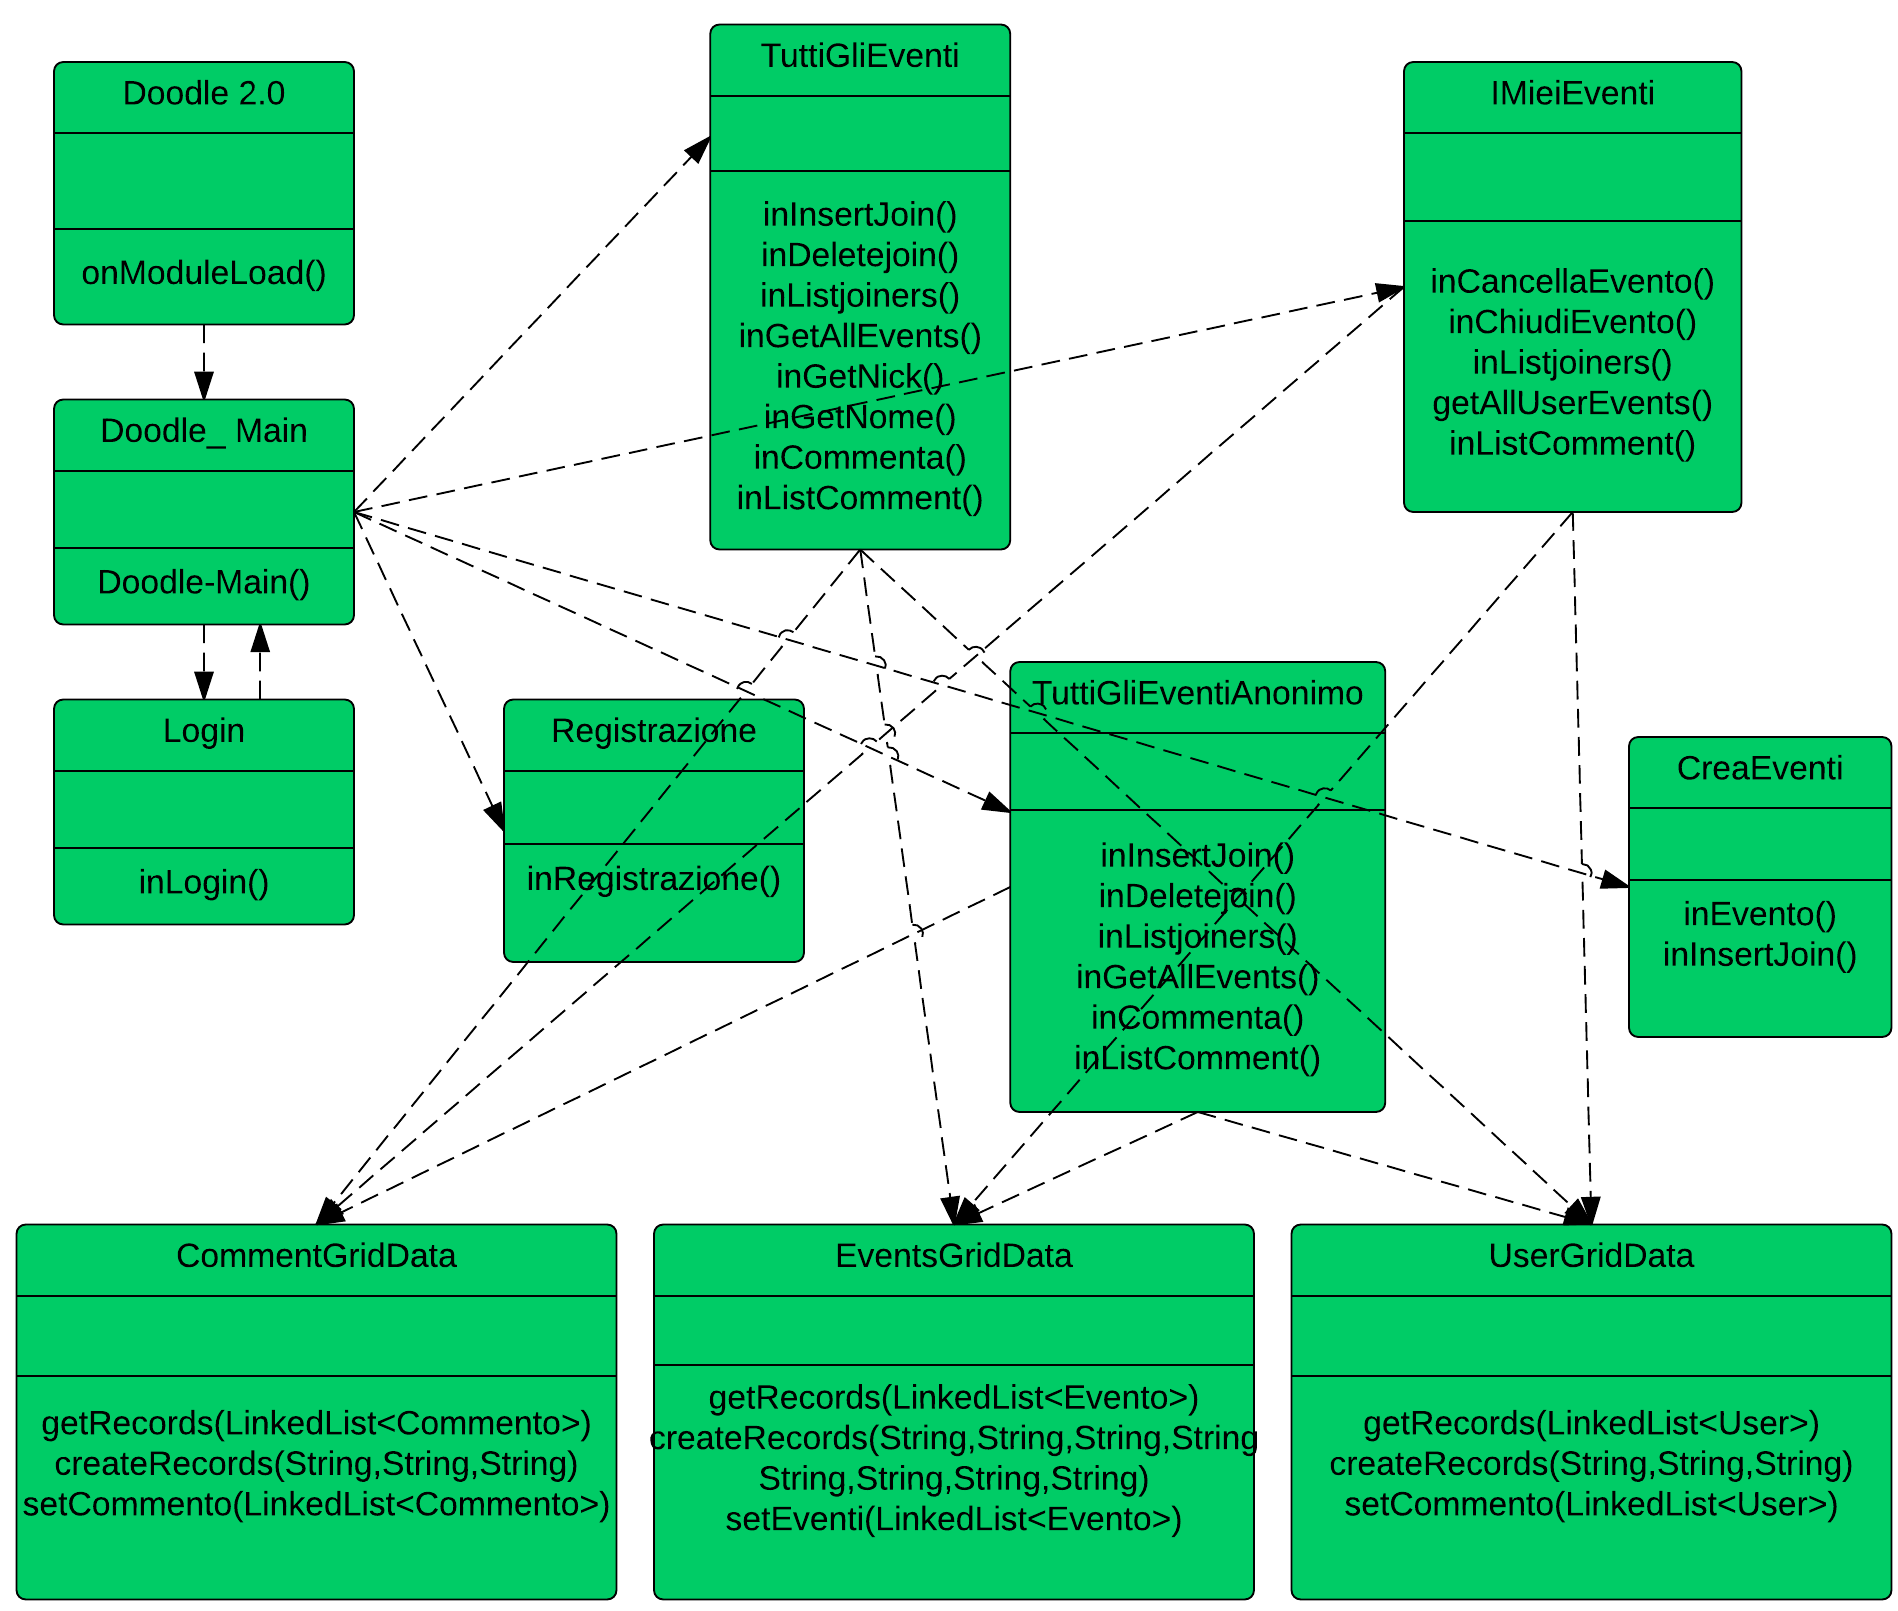
\includegraphics[]{img/classi/diagrammaclassi2.png}
	\caption{Diagramma delle classi Doodle 2.0}
	\label{fig:diagclassi2}
\end{figure}
\chapter{Diagramma di sequenza}
\section{Diagramma di sequenza}
\begin{figure}[H]
	\centering
	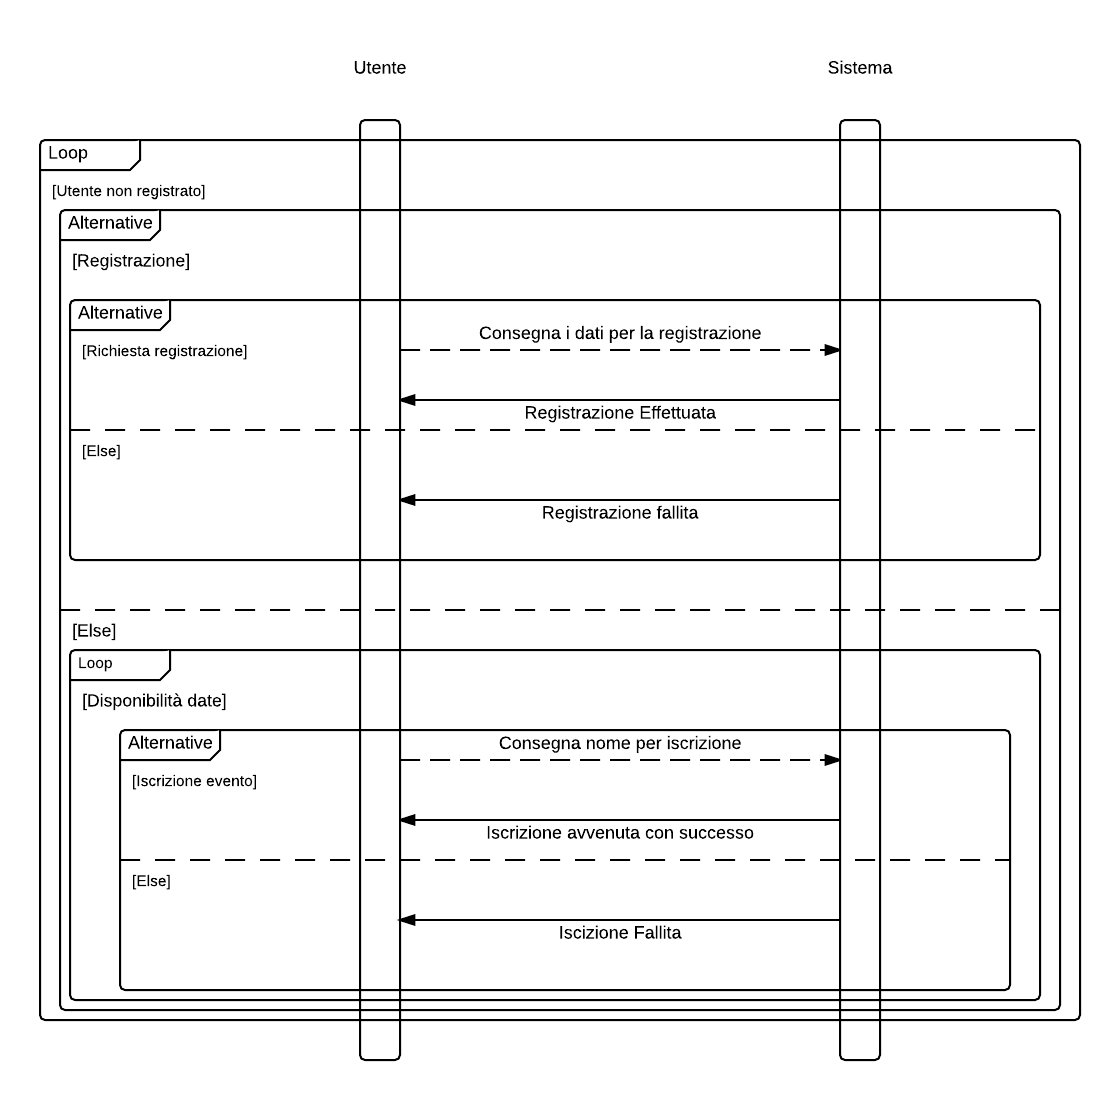
\includegraphics[scale=0.30]{img/sequenza.png}
	\caption{Diagramma di Sequenza}
	\label{fig:sequenza}
\end{figure}
\chapter{Diario}
\section{Diario Doodle 1.0}
\begin{itemize}
\item 3 Settembre: 	
	\begin{itemize}
			\item Identicazione dei primi dubbi sulle speciche;
			\item Identicazione e cenni all'utilizzo dei tool: \\
	
	\href{https:www.lucidchart.com}{Lucidchart.com} per i diagrammi;
	\end{itemize}
	
\item 4 Settembre:
	\begin{itemize} 
		\item Individuazione dei vari scenari possibili.
		\item Prima stesura dell' Use Case diagram. 
		
	 \end{itemize}

\item 10 settembre:
\begin{itemize} 
	\item Prodotte le bozze per il Glossario di progetto e diagrammi dei casi d'uso.
	\item Revisione dei diagrammi dei casi d'uso
	\item Inizio dei diagrammi delle attività.
	
\end{itemize}

\item 14 settembre:
\begin{itemize} 
	\item Diagrammi delle attività.
\end{itemize}

\item 16 settembre:
\begin{itemize} 
	\item Sviluppo dei  diagrammi delle attività. 
	\item Effettuate delle piccole correzzioni sui diagrammi dei casi d'uso.
	
\end{itemize}

\item 18 settembre:
\begin{itemize} 
	\item Fine dei diagrammi delle attività ed inizio il diagramma delle classi.
	
\end{itemize}
\item 20 settembre:
\begin{itemize} 
	\item Diagramma di sequenza.
	
\end{itemize}
\item 21 settembre:
\begin{itemize} 
	\item Analisi dei requisiti funzionali.
	
\end{itemize}

\item 25 settembre:
\begin{itemize} 
	\item Ultima revisione della documentazione , sono stati corretti gli ulrimi errori.
	
\end{itemize}

\item 28 settembre:
\begin{itemize} 
	\item Prima stesura del progetto.
	\item Inizio stesura codice e progettazzione dell'interfaccia.
	
\end{itemize}

\item 2 ottobre:
\begin{itemize} 
	\item Scelta della gestione del db. In un primo momento scelto MYSQL.
	\item Inizio Stesura codice server.
	\item Inizio stesura query (file querymethods -> Doodle 1.0)
	\item Inizio Stesura codice client.
	
\end{itemize}
\item 3...5..8 ottobre:
\begin{itemize} 
	\item Continuo la stesura del codice server e client.
	\item Aggiunte funzioni di controllo.
	
\end{itemize}

\item 10 Ottobre
\begin{itemize} 
	\item Primi test dell'applicazione.
	\item Correzione dei bug.
	
\end{itemize}

\item 11 Ottobre
\begin{itemize} 
	\item Stesura codice del client.
	\item Nuovi test.
	
\end{itemize}

\item 15 Ottobre
\begin{itemize} 
	\item Stesura codice del client e server.
	\item Nuovi test.
	
\end{itemize}

\item 15 Ottobre
\begin{itemize} 
	\item Debug.
	\item Nuovi test.
	
\end{itemize}

\item 16 Ottobre
\begin{itemize} 
	\item Ultimate le ultime modiche sulla parte server e client del progetto.
	\item Test della applicazione.
	\item Revisione della documentazione.
	
\end{itemize}	
\end{itemize}

\section{Diario Doodle 2.0}
Dopo aver scopetro che si consigliava usare MapDb per la gestione del DB ho ripreso Doodle 1.0 per apportare le modifiche richieste. Le modifiche sono state apportate facendo attenzione a non modificare , se non nei casi di obbligo, la parte client side. In seguito il diario del porting a mapdb:\\
\begin{itemize}
	\item 1 Novembre: 	
	\begin{itemize}
		\item Inzio a pensare a come introdurre MapDB.
		\item Identicazione di tutte le funzioni necessarie alla gestione del db (openDb(), commit(), rollback(), etc.  )
	\end{itemize}
	
	\item 2...3...4 Novembre: 	
	\begin{itemize}
		\item Modifiche alla documentazione.
		\item Inizio modifiche lato server.
		\item Creazione ServerDoodle.
	\end{itemize}
	\item 5...9 Novembre: 	
	\begin{itemize}
		\item Scrittura ServerDoodle.
	\end{itemize}
	
	\item 10 Novembre: 	
	\begin{itemize}
		\item Scrittura ServerDoodle.
		\item Piccole modifiche lato client.
	\end{itemize}
	
	\item 11 Novembre
	\begin{itemize}
		\item Modifca ServerDoodle.
		\item Introdotta nuova grafica.
	\end{itemize}
	
		\item ...15 Novembre
		\begin{itemize}
			\item Debug ServerDoodle.
			\item Nuova grafica.
			\item Test junit.
		\end{itemize}
		
		\item 17 Novembre
		\begin{itemize}
			\item Test junit.
			\item Rimozione codice inutilizzato.
		\end{itemize}
		
	\end{itemize}
	
	
	
\chapter{Ciclo di sviluppo}	
\section{Ciclo di sviluppo}	
La metodologia suggerita prevede una fase di analisi monolitica, che produca come artefatti una modellazione dei casi d'uso, attività, classi e sequenza e una di realizzazione iterativa ed incrementale ispirata ad una delle varie metodologie agili. In prima fase, quindi, ho sviluppato il Documento di Analisi con i vari diagrammi. In seguito, poi, mi sono dedicato alla progettazione dell'applicazione. Dopodiche mi sono dedicato allo sviluppo della prima release dell'applicazione andando a eliminare i problemi e le incongruenze sorte, risolvendo i problemi ad alto rischio prima e tralasciando quelli banali. Cosi facendo ho avuto modo di consentire un rapido sviluppo di versioni man mano più complete dell'applicazione. Una volta testato il lato server, mediante utilizzo di Junit mi sono dedicatoai test. Infine ho dato spazio all'aspetto grafico curandone i dettagli. Il tutto è stato frequentemente "committato" su github \href{https://github.com/jgemmy/Doodle}{Github} e \href{https://bitbucket.org/jgemmy/doodle}{Bitbucket}.Questa relazione (pdf) è stata scritta in Latex. Caricati i file .tex sui git.

\end{document}
